\documentclass{article}

\usepackage{graphicx}
\usepackage{tikz}
\usepackage{tikzsymbols}
\usetikzlibrary{calc,patterns,shapes.geometric}
\pagestyle{empty}
\usepackage[margin=0pt]{geometry}
\geometry{papersize={14in,12in}}

\def\centerarc[#1](#2)(#3:#4:#5){\draw[#1] ($(#2)+({#5*cos(#3)},{#5*sin(#3)})$) arc (#3:#4:#5);}

\begin{document}
	\begin{figure}
		\centering
		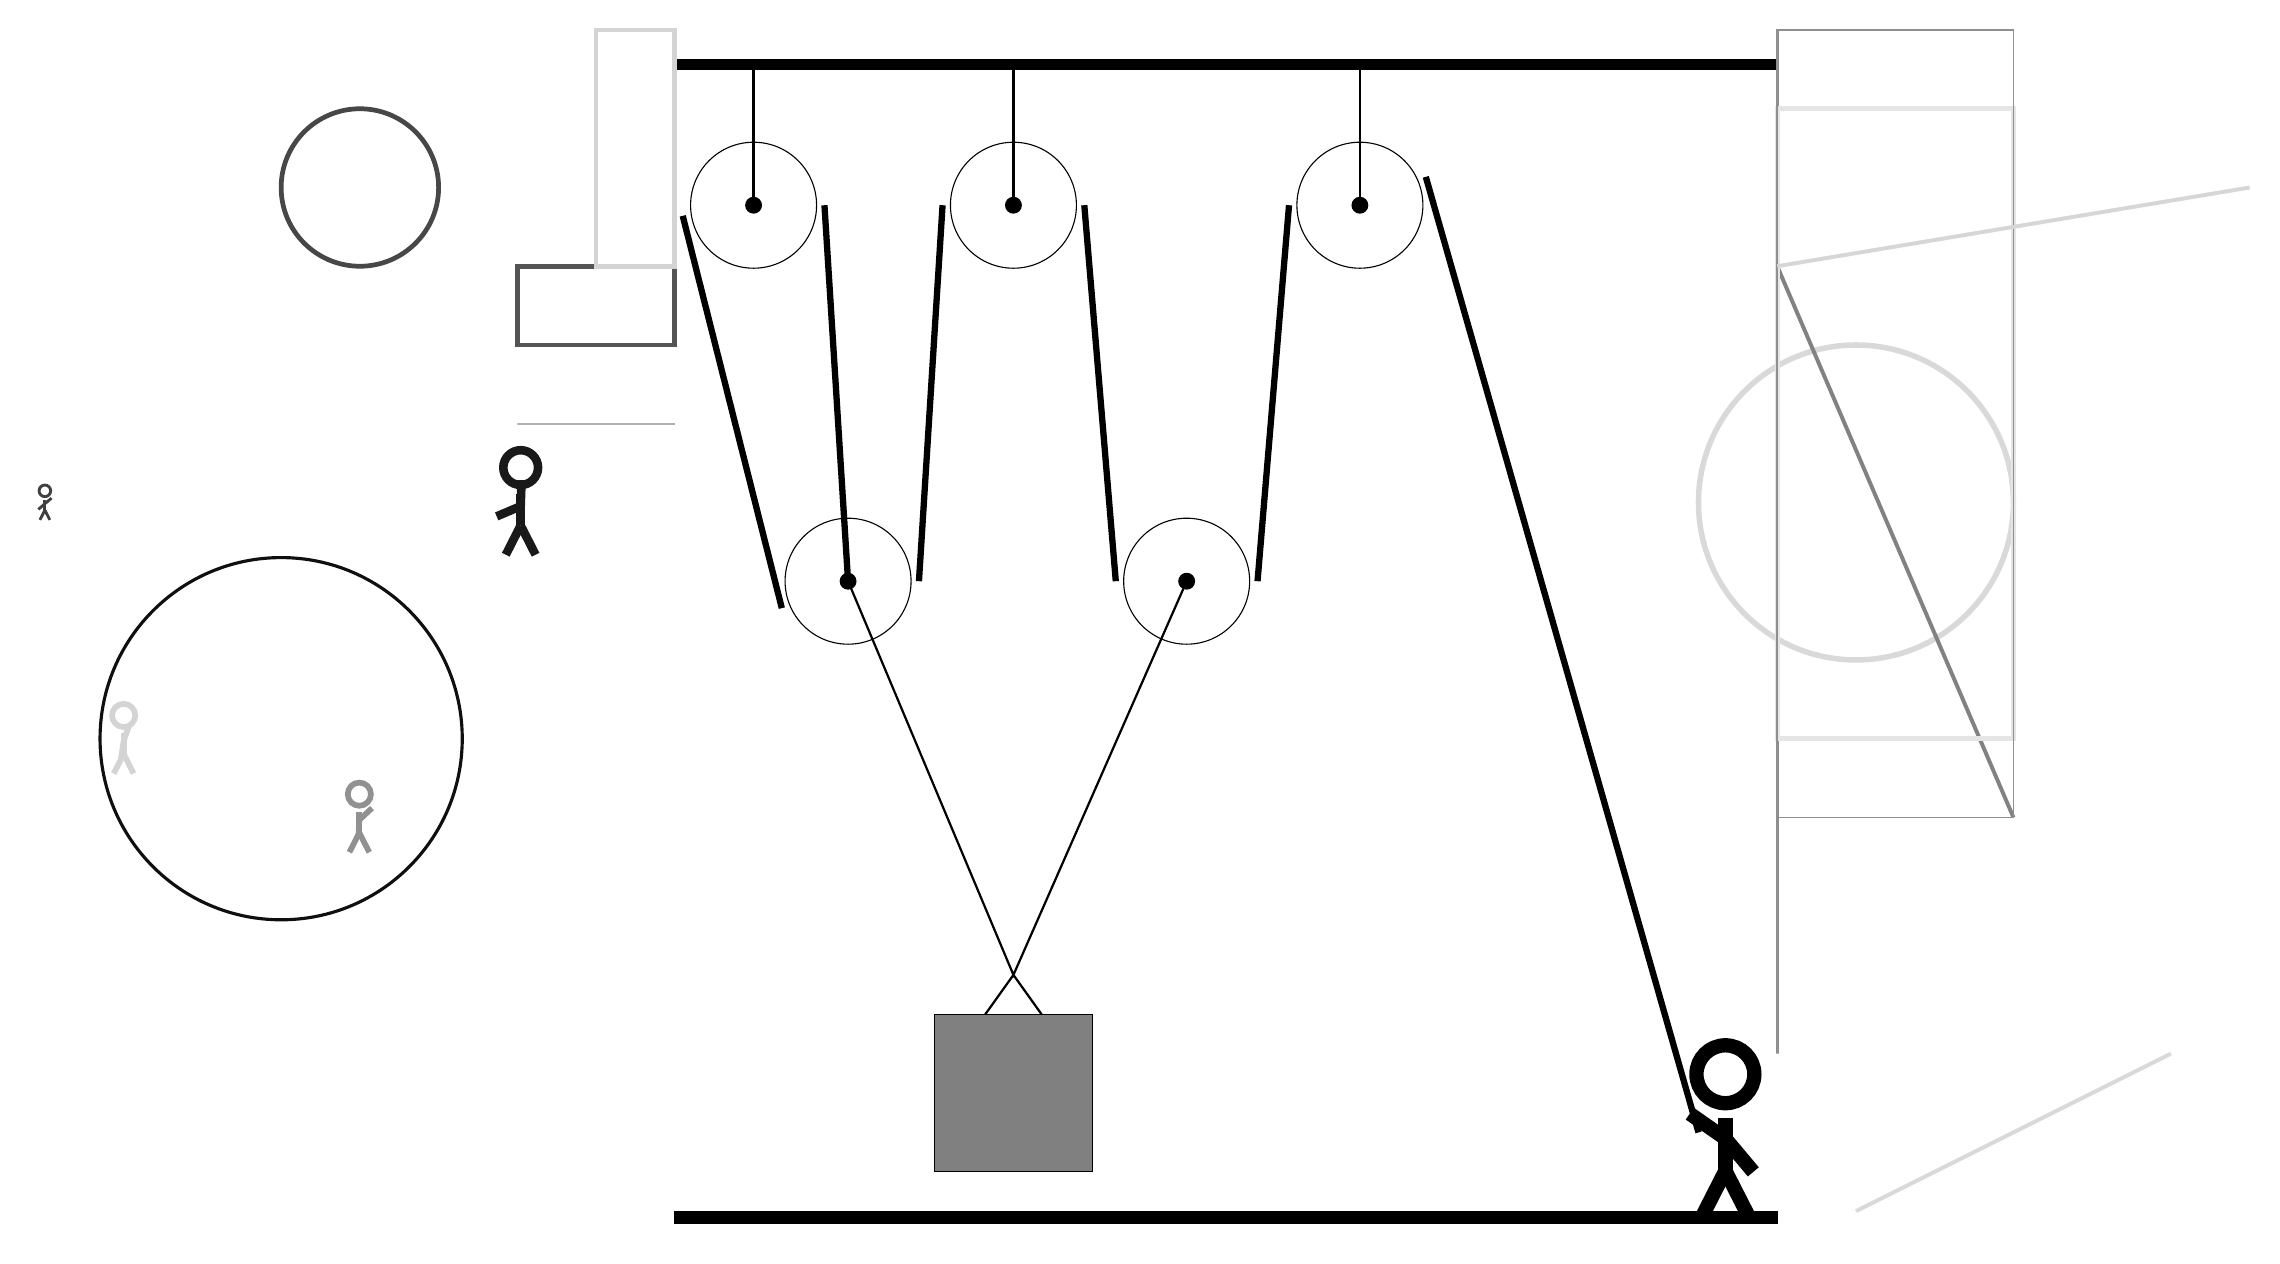
\begin{tikzpicture}
			%%%%% START %%%%%
			
			\draw[fill=black] (-2, 11.5) rectangle (12, 11.625);
			
			\draw (-1, 9.775) circle (0.8);
			\draw[fill=black] (-1, 9.775) circle (0.1);
			\draw[thick] (-1, 9.775) -- (-1, 11.5);
			
			\draw (2.3, 9.775) circle (0.8);
			\draw[fill=black] (2.3, 9.775) circle (0.1);
			\draw[thick] (2.3, 9.775) -- (2.3, 11.5);
			
			\draw (6.7, 9.775) circle (0.8);
			\draw[fill=black] (6.7, 9.775) circle (0.1);
			\draw[thick] (6.7, 9.775) -- (6.7, 11.5);
			
			\draw (0.2, 5) circle (0.8);
			\draw[fill=black] (0.2, 5) circle (0.1);
			
			\draw[line width=0.6mm, color=black!37] (12, 3) rectangle (12, 4);
			
			\draw[line width=0.6mm, color=black!67] (-4, 9) rectangle (-2, 8);
			\draw [line width=0.7mm, color=black!15](13, 6) circle (2.0);
			\draw[line width=0.5mm, color=black!49](15, 2) -- (12, 9);
			\draw[line width=0.6mm, color=black!17] (-2, 12) rectangle (-3, 9);
			
			\draw[line width=0.4mm, color=black!44] (12, -1) rectangle (12, 12);
			\node[line width=0.6mm, color=black!90] at (-4, 6) {\Strichmaxerl[6][23][88]};
			\draw[line width=0.2mm, color=black!31] (-2, 7) rectangle (-4, 7);
			\node[line width=0.2mm, color=black!17] at (-9, 3) {\Strichmaxerl[4][81][71]};
			\node[line width=0.7mm, color=black!75] at (-10, 6) {\Strichmaxerl[2][41][40]};
			\draw [line width=0.6mm, color=black!72](-6, 10) circle (1.0);
			
			\node[line width=0.2mm, color=black!43] at (-6, 2) {\Strichmaxerl[4][87][43]};
			\draw [line width=0.4mm, color=black!94](-7, 3) circle (2.3);
			
			\draw[line width=0.6mm, color=black!10] (12, 11) rectangle (15, 3);
			\draw[line width=0.2mm, color=black!44] (12, 12) rectangle (15, 2);
			\draw[line width=0.5mm, color=black!15](17, -1) -- (13, -3);
			
			\draw[line width=0.5mm, color=black!16](12, 9) -- (18, 10);
			
			
			\draw (4.5, 5) circle (0.8);
			\draw[fill=black] (4.5, 5) circle (0.1);
			
			\draw[thick] (0.2, 5) -- (2.3, 0)  -- (4.5, 5);
			\draw[thick]  (1.8, -0.7) -- (2.3, 0) -- (2.8, -0.7);
			\draw[fill=black!50] (1.3, -0.5) rectangle (3.3, -2.5);
			
			\draw[line width=0.8mm] (0.2, 5) -- (-0.1, 9.775);
			\centerarc[line width=0.8mm](-1, 9.775)(0:200:0.9);
			\draw[line width=0.8mm] (-1.9, 9.64) -- (-0.6415, 4.658);
			\centerarc[line width=0.8mm](0.2, 5)(200:360:0.9);
			\draw[line width=0.8mm](1.1, 5) -- (1.4, 9.775);
			\centerarc[line width=0.8mm](2.3, 9.775)(0:180:0.9);
			\draw[line width=0.8mm] (3.2, 9.775) -- (3.6, 5);
			\centerarc[line width=0.8mm](4.5, 5)(180:360:0.9);
			\draw[line width=0.8mm] (5.4, 5) -- (5.8, 9.775);
			\centerarc[line width=0.8mm](6.7, 9.775)(20:180:0.9);
			\draw[line width=0.8mm](7.537, 10.135)  -- (11, -2);
			
			\node at (11.3, -2) {\Strichmaxerl[10][-35][-50]};
			
			\draw[fill=black] (-2, -3) rectangle (12, -3.15);
			
			%%%%% END %%%%%
		\end{tikzpicture}
	\end{figure}	
\end{document}